% Platzhalter


% Variablen

% Titel der Abschlussarbeit
\newcommand{\myTitle}{Eine Vorlage für Bachelor- und Masterarbeiten}

% Vor- und Nachname
\newcommand{\myAuthor}{Au Tor}

% Datum der Abgabe
\newcommand{\myDate}{1. Januar 2024}

% Ort
\newcommand{\myOrt}{Emden}

% Matrikelnummer
\newcommand{\myMatrikelnummer}{12345678}

%%%%%%%%%%%%%%%%%%%%%%%%%%%%%%%%%%%%%%%%%%%%%%%%%%%%%%%%%%%%%%%%%%%%%%

\documentclass
[
    ngerman,
    headsepline, % Linie in Kopfzeile
    automark,
    listof=totoc, % Verzeichnisse im Inhaltsverzeichnis aufführen
    bibliography=totoc, % Literaturverzeichnis im Inhaltsverzeichnis aufführen
    oneside, % Einseitig
    appendixprefix, % Das Wort "Anhang" vor dem Buchstabe des Anhangs ergänzen
    numbers=noenddot, % Kein Punkt nach Kapitelnummer
    parskip
]
{scrbook}

% Laden der Pakete
\usepackage[utf8]{inputenc}
\usepackage[T1]{fontenc}
\usepackage{lmodern}

% glqq
\usepackage[ngerman]{babel}

% Required for inserting images
\usepackage{graphicx}

% Beliebige Schriftgrößen verwenden
% https://ctan.org/pkg/anyfontsize
\usepackage{anyfontsize}

\usepackage{scrlayer-scrpage}

% Layout von itemize, enumerate und description anpassen
% https://ctan.org/pkg/enumitem
\usepackage{enumitem}

% Verwenden von \theauthor etc.
%\usepackage{titling}

% Muss vor Package natbib geladen werden
\usepackage{apacite}

% Für cite
\usepackage{natbib}
\usepackage{citeref}
%\usepackage{varioref}

\usepackage{hyperref}


% Muss nach Package hyperref geladen werden
\usepackage[acronym,toc]{glossaries}

% Code
\usepackage{listings}

% Einfärben der Hyperlinks, anstelle der Boxen...
\usepackage{xcolor}
\hypersetup{
    colorlinks,
    linkcolor={red!50!black},
    citecolor={blue!50!black},
    urlcolor={blue!80!black}
}


\clearpairofpagestyles

% Anpassen der Kopfzeile: Kapitel links, Seitenzahl rechts
\ihead[]{\headmark}
\ohead[]{\pagemark}

\pagestyle{scrheadings}

% Kopfzeile auch auf Seiten, auf denen ein Kapitel anfängt
\renewcommand*\chapterpagestyle{scrheadings}

% Grafikordner auf "images/" setzen
\graphicspath{{images/}}

% New colors defined below
\definecolor{codegreen}{rgb}{0,0.6,0}
\definecolor{codegray}{rgb}{0.5,0.5,0.5}
\definecolor{codepurple}{rgb}{0.58,0,0.82}
\definecolor{backcolour}{rgb}{0.95,0.95,0.92}

% Code listing style named "mystyle"
\lstdefinestyle{mystyle}{
  backgroundcolor=\color{backcolour},
  commentstyle=\color{codegreen},
  keywordstyle=\color{magenta},
  numberstyle=\tiny\color{codegray},
  stringstyle=\color{codepurple},
  basicstyle=\ttfamily\footnotesize,
  breakatwhitespace=false,         
  breaklines=true,                 
  captionpos=b,                    
  keepspaces=true,                 
  numbers=left,                    
  numbersep=5pt,                  
  showspaces=false,                
  showstringspaces=false,
  showtabs=false,                  
  tabsize=2
}

\lstset{style=mystyle}


\newacronym{gcd}{GCD}{Greatest Common Divisor}

\newacronym{lcm}{LCM}{Least Common Multiple}

\newglossaryentry{maths}
{
    name=mathematics,
    description={Mathematics is what mathematicians do}
}

\newglossaryentry{latex}
{
    name=latex,
    description={Is a markup language specially suited for scientific documents}
}

\newglossaryentry{formula}
{
    name=formula,
    description={A mathematical expression}
}


\makeglossaries

\begin{document}

% Anfang des Dokuments
\frontmatter

\begin{titlepage}

\begin{center}

\begin{figure}[tbh]
 \centering
 
\includegraphics[width=0.5\textwidth]{hs-emden-leer_logo.png}
\end{figure}

\vspace{1.5cm}

{
 \fontsize{24.88}{28}\selectfont
 \myTitle\\[0.5cm]
}

\fontsize{12}{12}\selectfont

\vspace{1.5cm}

Bachelor-/Masterarbeit\\
zur Erlangung des akademischen Grades Y\\
im Studiengang X\\
des Fachbereichs Technik\\
an der Hochschule Emden/Leer

\vspace{0.5cm}

Eingereicht von\\
\myAuthor\\
Matrikelnummer: \myMatrikelnummer

\vspace{0.5cm}

Erstprüfer:\\
Prof. Dr. Thies Pfeiffer\\
Hochschule Emden/Leer\\
Constantiaplatz 4\\
26723 Emden\\

\vspace{.2cm}

ZweitprüferIn:\\
Vorname Nachname\\
Firma / Institution\\
Straße Nummer\\
PLZ Ort

\vspace{0.5cm}

\myOrt, den \myDate

\end{center}
\end{titlepage}


\cleardoublepage

% Römische Zahlen in Groß
\pagenumbering{Roman}

\chapter{Abstract}

Kurzfassung auf Englisch.

\chapter{Kurzfassung}

Kurzfassung auf Deutsch.

\chapter{Danksagung}

Danke an …


\tableofcontents
\listoffigures
\listoftables
\printglossary[type=\acronymtype,title=Abkürzungsverzeichnis]
\printglossary[title=Glossar]

\cleardoublepage

%\pagenumbering{arabic}

% Hauptteils des Dokuments
\mainmatter

\chapter{Einleitung}

Diese \LaTeX-Vorlage soll als Leitlinie und Anhaltspunkt für das Schreiben von Abschlussarbeiten dienen. Zum einen zeigt die Vorlage eine typische Struktur einer Abschlussarbeit auf, an der sich viele Arbeiten orientieren. Zum anderen gibt diese Vorlage gleichzeitig Tipps und Hinweise sowohl was die Strukturierung als auch was mögliche Technologien, insbesondere \LaTeX-Pakete, angeht.

Typischer Umfang der Einleitung: 1-3 Seiten.

\section{Motivation}

Der wesentliche Abschnitt der Einleitung ist die Motivation, in der die Arbeit in einen Kontext gesetzt wird. Wichtig ist dabei vor allem, den Leser abzuholen und relativ zügig in das Thema einzuführen. Dazu eigenen sich oft auch Bilder oder Skizzen sehr gut. In vielen Fällen kann dies durch ein konkretes Beispiel gelingen.

Die Motivation darf dabei ruhig auf eine größere Vision hin abzielen, auch wenn im Rahmen der Abschlussarbeit dann vielleicht nur ein bestimmter Aspekt oder eine prototypenhafte Umsetzung realisiert werden kann. Es ist aber wichtig, dem Leser den Gesamtkontext zu vermitteln, damit dann die einzelne Leistung besser eingeordnet werden kann.

\section{Zielsetzung}

In diesem Abschnitt sollte die Zielsetzung der Arbeit genau entwickelt werden. Hier bietet es sich an, die Zielsetzungen z.B. als Aufzählung an dieser Stelle einzuführen, damit später auf die einzelnen Zielsetzungen verwiesen werden kann.

\begin{enumerate}[labelsep=1ex]
    \renewcommand{\labelenumi}{\textbf{Z\theenumi.}}
    \item Diese Vorlage soll den grundlegenden Aufbau einer Abschlussarbeit aufzeigen.
    \item Diese Vorlage soll relevante \LaTeX-Beispiele für die eigene Arbeit liefern.
\end{enumerate}

\subsection{Hop oder Top?}
Eine grundsätzliche Frage, die sich bei allen Projekten stellt, ist: wie kann man den Erfolg eines Projektes bestimmen? Für das eigene Arbeiten ist es hilfreich, sich darüber auch beim eigenen Projekt frühzeitig Gedanken zu machen und die Zielsetzungen auch so zu formulieren, dass man es später leicht, den Erfolg zu prüfen.

Eine Formulierung wie {\em 'Es soll ein intuitives Benutzerinterface für gestenbasierte Interaktion entwickelt werden.'} klingt zwar cool, lässt aber die Frage nach der Bestimmung des Erfolgs offen. Eigenschaften wie {\em intuitiv} oder {\em natürlich} zu messen fällt relativ schwer. Eine bessere Variante könnte sein: 

{\em 'Es soll ein intuitives Benutzerinterface für gestenbasierte Interaktion entwickelt werden, dass sich dadurch auszeichnet, dass die Handformen während der gesamten Interaktion richtig bestimmt werden können und eine geringere Anzahl an Fehlinterpretationen erreicht wird als mit dem vom Hersteller mitgelieferten Algorithmus.'}

In dieser Variante wird zum einen die Methode eines Vergleichs mit einem existierenden Ansatz genutzt, zum anderen eine Beschreibung der Abdeckung einer vorgegebenen Situation. Andere Methoden zur Bewertungen können Usability-Tests sein, oder bestimmte Performanz-Maße (höher, schneller, weiter).

Ein wichtiger Vorteil von einer solchen Quantifizierung einer Aufgabenstellung ist es, dass man auch bereits bei der eigenen Entwicklung kontinuierlich messen kann, wie gut das entwickelte System aktuell dasteht.

Von der möglichen Messbarmachung sollte man sich jedoch auch nicht zu sehr einschränken lassen. Manchmal sind es aber auch einfach nur kleine Formulierungsänderungen, die plötzlich eine Quantifizierung ermöglichen.

\section{Aufbau der Arbeit}

In diesem Abschnitt wird schließlich kurz erklärt, wie der weitere Aufbau der Arbeit ist. Welche Kapitel kommen jetzt noch und mit welchem Thema beschäftigen sich diese? Damit soll dem Leser ein kurzer Überblick gegeben werden. Insbesondere bei einer Bachelorarbeit sollte dieser Abschnitt jedoch sehr knapp gefasst werden.

\chapter{Stand der Forschung / Stand der Technik}

In diesem Kapitel soll der Bezug der Arbeit zum aktuellen Stand der Forschung, bzw. zum Stand der Technik, je nach Ausrichtung und Schwerpunkt der Arbeit, verdeutlicht werden. Dazu werden entsprechende Vorarbeiten oder alternative Ansätze vorgestellt und diskutiert. Ziel ist es, den Ansatzpunkt der Arbeit genauer zu bestimmen und etwaige Entscheidungen im späteren Verlauf des Textes zu fundieren.

Dieses Kapitel kann je nach Thema der Arbeit {\emph Stand der Forschung} oder
{\emph Stand der Technik} heißen. In jedem Kapitel ist es wichtig, wie hier
geschehen zu Beginn kurz zu erläutern, um was es in diesem Kapitel geht.

Typischer Umfang des Stands der Forschung: 2-4 Seiten BA, 10-15 Seiten MA.

\section{Richtig zitieren}

In den letzten Jahren gab es auch in der Öffentlichkeit einiges an Diskussion zum Thema {\em Richtiges Zitieren}. Hier die wesentlichen Punkte:

\begin{itemize}
     \item Wenn Aussagen gemacht werden, dann sollten diese wenn möglich durch ein Zitat (eine Literaturstelle) belegt werden.
     \item Alle Literaturstellen werden im Anhang im Literaturverzeichnis gesammelt und über einen entsprechenden Befehl im Text einbezogen (Bibtex ist euer Freund).
     \item Der Teil des Textes, auf den sich die Literaturreferenz bezieht, sollte deutlich werden. 
 
    \begin{itemize}
        \item Ist es eine bestimmte Aussage, dann kommt die Referenz ans Ende des Satzes: \glqq Blickbewegungen in realen Umgebungen kann man mittels Bildverarbeitung auf der Szenenkamera quantifizieren~\citep{3}.\grqq\ Alternativ hätte man es auch anders schreiben können: \glqq \citet{3} zeigen, wie man Blickbewegungen in realen Umgebungen mittels Bildverarbeitung auf der Szenenkamera quantifizieren kann.\grqq 
        \item Oder, bei mehreren Teilsätzen: \glqq Während im ersten Fall einfach Boxen gezeichnet werden~\citep{3}, können andere Heatmaps auf 3D Objekten zeichnen~\citep{4}.\grqq bzw. \glqq Während \citet{3}  einfach Boxen zeichnen, zeichnen \citet{4} Heatmaps auf 3D Objekten.\grqq
    \end{itemize}
 
    \item In der Informatik nutzen wir nur in Ausnahmefällen wörtliche Zitate. Wichtiger sind bei uns Zusammenfassungen und Bewertungen der Aussagen anderer.
\end{itemize}

\section{Breit oder Tief?} 

Gerade in diesem Kapitel sehen sich viele Autoren in einem Zwiespalt. Auf der
einen Seite gibt es sehr viele spannende Inhalte, die man sich vielleicht selbst
erst kürzlich erarbeitet hat. Da macht es natürlich Spaß und dient auch dem
eigenen Verständnis, diese hier wieder zu geben. Allerdings schreibt man dann
primär über Dinge, die andere getan haben und nicht über das, was man selbst
geleistet hat. Ein klarer Fokus bei allen Inhalten in der Abschlussarbeit sollte
jedoch auf der {\normalfont \bfseries eigenen Leistung} liegen. 

Die eigene Leistung kann zum Beispiel darin liegen, aus der vorhandenen
Literatur punktgenau heraus zu arbeiten, was die genauen Unterschiede in den Ansätzen
verschiedener relevanter Algorithmen sind, oder wie sich bestehende
Veröffentlichungen kategorisieren lassen, etc. Die eigene Leistung ist also die
Arbeit mit den Texten, das genauere Hinsehen, und weniger das einfache Berichten über die Texte. Dazu werden die Texte exakt referenziert, so dass man eben nicht mehr gezwungen ist, alle auch nur entfernt relevanten Inhalte hier wieder zu geben.

Der Platz in diesem Kapitel sollte also primär für einen guten breiten Überblick dienen, der dann ins Detail geht, wenn die Stellen behandelt werden, an denen die vorliegende Arbeit ganz konkret ansetzt bzw. für die die vorliegende Arbeit Alternativen erarbeitet.

\section{Zusammenfassung} 

Jedes Kapitel sollte mit einer eigenen Zusammenfassung abschließen (vielleicht
ausgenommen dem einleitenden Kapitel). Der einleitende Text des Kapitels und die
Zusammenfassung bilden zugleich eine Klammer um das Kapitel und zeigen einen
roten Faden im Übergang zwischen den Kapiteln auf. 

Das wesentliche bei der Zusammenfassung insbesondere im Kapitel {\emph Stand der
Forschung} ist es, das im Kapitel beschriebene in eigenen Worten kurz und prägnant
darzustellen und in Bezug zur eigenen Arbeit zu setzen.

Es könnte in der Zusammenfassung zum Beispiel stehen: \glqq Wie X und Y gezeigt
haben, ist noch offen, wie... In dieser Arbeit soll diese Frage so und so
angegangen werden.\grqq Oder \glqq Wie gezeigt werden konnte, gibt es derzeit für X
noch keine (zufriedenstellende) Lösung...\grqq.

\chapter{Konzeption}

Im Kapitel {\em Konzeption} beginnt jetzt die Darstellung der eigenen Arbeit. Dieses Kapitel stellt das Bindeglied zwischen Zielsetzung, Stand der Forschung und der eigentlichen Umsetzung dar. Zusammen mit Implementierung und Evaluation macht die Konzeption den Hauptteil der Arbeit aus.

Typischer Umfang der Konzeption: 5-10 Seiten BA, 15-20 Seiten MA.

\section{Konzeption oder Implementierung}

Vielen fällt es schwer, zwischen Konzeption und Implementierung zu unterscheiden. Das ist auch gar nicht so einfach, aber ein paar Leitlinien können die Entscheidung leichter machen:

\begin{itemize}
    \item Die Konzeption sollte von konkreten technischen Details abstrahieren und sich auf das Kernproblem fokussieren.
    \item Handelt es sich z.B. im Kern um einen Algorithmus, würde man diesen in der Konzeption auf einer abstrakten Ebene beschreiben (z.B. Pseudocode) und in der Implementierung dann auf konkrete Aspekte und Lösungen mittels bestimmter Programmiersprachen, -methoden, oder Bibliotheken eingehen.
    \item In anderen Fällen geht es vielleicht um eine Architektur, dann würde diese mit Mitteln wie z.B. UML in der Konzeption entwickelt und dann in der Implementierung im Detail dargestellt werden.
    \item Steht man vor der Entscheidung, ob etwas eher in die Konzeption oder in die Implementierung gehört, dann kann man dies oft über die folgende Frage entscheiden: {\em Muss jemand, der ein ähnliches Problem unter anderen Bedingungen bearbeitet, das wissen?} Wenn ja, dann gehört es eher in die Konzeption, falls es sich um etwas handelt, was man nur für die konkrete Anwendung wissen muss, dann gehört es eher in die Implementierung. In die Konzeption gehören eher die Aspekte, die etwas abstrakter sind und die wahrscheinlich länger von Bedeutung sind. In die Implementierung gehört alles das, was zum konkreten Verständnis der eigenen Umsetzung notwendig ist und was sich nicht aus der abstrakten Sicht erschließt.
\end{itemize}

\chapter{Implementierung}

Die Implementierung beschreibt ganz grundlegende technische Details der Umsetzung. Das kann von konkreten Entscheidungen, wie der Wahl einer bestimmten Programmiersprache oder bestimmter Software-Bibliotheken, bis hin zu Auszügen aus dem Programmcode gehen.

Typischer Umfang der Implementierung: 5-10 Seiten BA, 15-20 Seiten MA.

\section{Installation, Nutzerdokumentation}

Unbedingt zur Implementierung gehört dann am Ende auch eine Beschreibung, wie man die Implementierung zu nutzen hat. Dazu gehört die Beschreibung, wie man die Implementierung bezieht und installiert, genauso wie eine kurze Beschreibung der Bedienung. Falls letztere zu umfangreich werden würde, aber notwendig ist, kann diese auch im Anhang aufgeführt und mit einem Verweis gearbeitet werden.

\chapter{Evaluation}

Wenn möglich, dann sollte jede Arbeit auch in irgendeiner Form evaluiert werden. Die Art der Evaluation kann sehr unterschiedlich sein, je nach Inhalt. Es kann eine Performanz-Messung sein, eine Nutzer-Studie, ein Vergleich oder auch die qualitative Bewertung dem Leser überlassen (z.B. bei Kunstalgorithmen).

Besonders praktisch ist es natürlich, wenn sich die Evaluation direkt aus den Zielsetzungen in der Einleitung ableiten lässt.

Wichtig ist, dass in der Evaluation erst einmal relativ neutral über die Art der Evaluation und die erzielten Ergebnisse berichtet werden sollte. Eine Bewertung findet erst später in der Diskussion statt.

Typischer Umfang der Evaluation: 2-3 Seiten BA, 5-10 Seiten MA.

\chapter{Diskussion}

Hier wird reflektiert, in welchem Umfang die Zielsetzungen der Arbeit erreicht werden konnten. In der Regel gelingt dies durch den Bezug auf die Evaluation.

Typischer Umfang: 1-2 Seiten.

\section{Ausblick}

Manchmal konnte im Rahmen einer Bachelor- oder Masterarbeit ein
wissenschaftliches Thema auch so tief bearbeitet werden, dass wir es auf einem
wissenschaftlichen Workshop oder einer Konferenz veröffentlichen konnten.

Für Themen aus dem Bereich Virtuelle oder Erweiterte Realität bietet sich dazu
zum Beispiel der jährlich stattfindende Workshop der Fachgruppe VR/AR der
Gesellschaft für Informatik an. \citet{Bluhm:Sonar:2009} ist nur ein Beispiel
von mehreren Veröffentlichungen aus unserer Gruppe.

\section{Test}
Kleine Tests, die später noch passend in den übrigen Text eingearbeitet werden.

\subsection{Tabelle}

Das ist \autoref{tab:example}.

\begin{table}[tbh]
 \centering
 \begin{tabular}{r|r}
 Test 1 & Test 2\\
 \hline
 abc & 123\\
 def & 456\\
 ghi & 789
 \end{tabular}
 \caption{Tabellen-Test}
 \label{tab:example}
\end{table}

\subsection{Bild}

Das ist \autoref{fig:example}.

\begin{figure}[tbh]
 \centering
 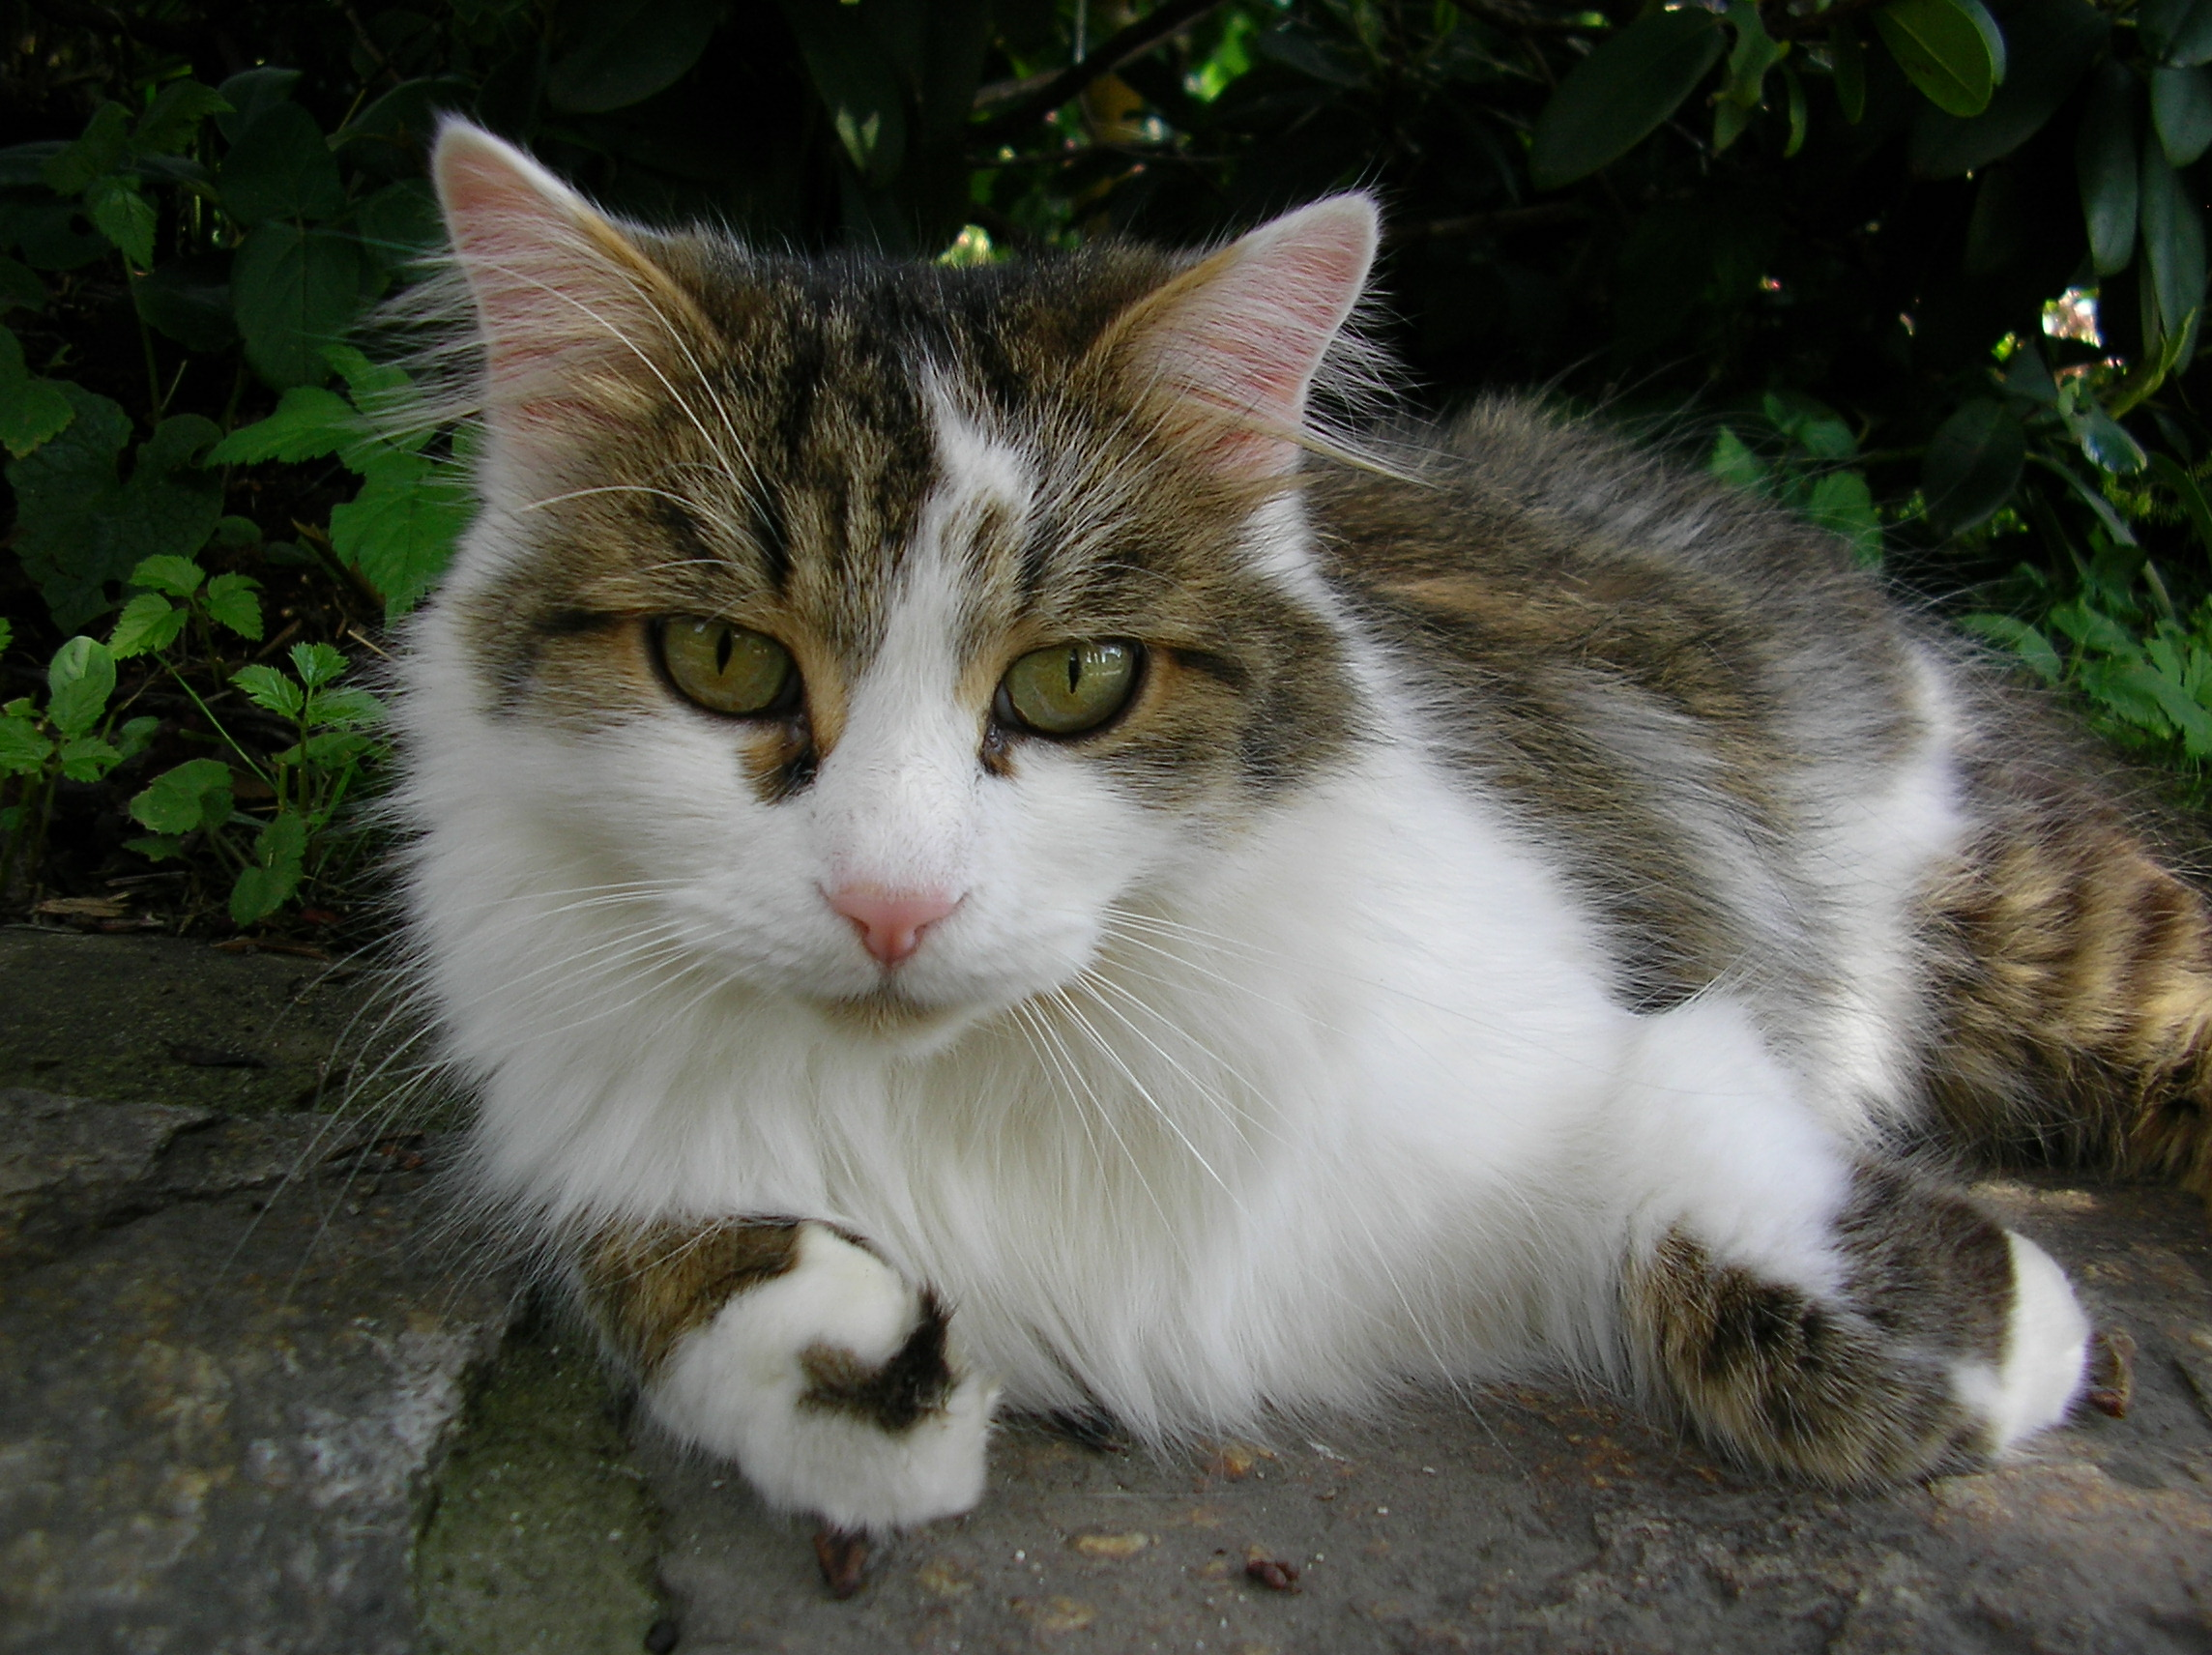
\includegraphics[width=0.5\textwidth]{Hauskatze_langhaar.jpg}
 \caption{Test-Bild}
 \label{fig:example}
\end{figure}

\subsection{Begriffe und Abkürzungen}
The \Gls{latex} typesetting markup language is specially suitable for documents that include \gls{maths}. \Glspl{formula} are rendered properly an easily once one gets used to the commands.

Given a set of numbers, there are elementary methods to compute its \acrlong{gcd}, which is abbreviated \acrshort{gcd}. This process is similar to that used for the \acrfull{lcm}.

\subsection{Mathematik}

\begin{equation}
 \sin \alpha = \left( \frac{a}{c} \right)
\end{equation}

\subsection{Code}

\autoref{lst:example} ist ein Code-Beispiel in Python.

\begin{lstlisting}[language=Python, caption=Code-Beispiel mit Python, label={lst:example}]
import numpy as np
    
def incmatrix(genl1,genl2):
    m = len(genl1)
    n = len(genl2)
    M = None #to become the incidence matrix
    VT = np.zeros((n*m,1), int)  #dummy variable
    
    #compute the bitwise xor matrix
    M1 = bitxormatrix(genl1)
    M2 = np.triu(bitxormatrix(genl2),1) 

    for i in range(m-1):
        for j in range(i+1, m):
            [r,c] = np.where(M2 == M1[i,j])
            for k in range(len(r)):
                VT[(i)*n + r[k]] = 1;
                VT[(i)*n + c[k]] = 1;
                VT[(j)*n + r[k]] = 1;
                VT[(j)*n + c[k]] = 1;
                
                if M is None:
                    M = np.copy(VT)
                else:
                    M = np.concatenate((M, VT), 1)
                
                VT = np.zeros((n*m,1), int)
    
    return M
\end{lstlisting}


\bibliographystyle{plainnat}
\bibliography{literature}

% Anhang
\appendix
%&%\chapter*{Anhang} % Ein Kapitel ohne Nummerierung
\addcontentsline{toc}{chapter}{Anhang} % Fügt das Anhang-Kapitel dem Inhaltsverzeichnis hinzu
%\addchap{Anhang}

\chapter{Test-Anhang}
% Versicherung bei Diplomarbeiten...

\section{Hinweise zum Layout}

\subsection{Druckseiten}

Zur besseren Korrektur der Arbeit sollten die im Prüfungsamt abzugebenden Exemplare einseitig gedruckt werden. Die Vorlage ist entsprechend ausgelegt. Für sich selbst, für Angehörige, etc, kann man später dann leicht noch mal eine beidseitig bedruckte Fassung erstellen.

\section{Zeitplanung}

\begin{itemize}
    \item Erfahrungsgemäß ist das Aufschreiben der Arbeit für die meisten mit am schwersten. Daher sollte damit frühzeitig begonnen werden. Spätestens zwei Wochen vor der Abgabe wird es allerdings allerhöchste Eisenbahn!
    \item Der Druck der Arbeit kann unter Umständen einen Tag in Anspruch nehmen, daher empfiehlt es sich, einen Abgabetermin ab Dienstag-Freitag zu wählen.
\end{itemize}

\cleardoublepage

\chapter{Test-Anhang 2}

Test

\cleardoublepage


% Anhang des Dokuments
\backmatter

\chapter{Erklärung}

Soweit meine Rechte berührt sind, erkläre ich mich einverstanden, dass die vorliegende Arbeit Angehörigen der Hochschule Emden/Leer für Studium / Lehre / Forschung unein-geschränkt zugänglich gemacht werden kann.

\vspace{2cm}

% Damit beide Kapitel auf einer Seite stehen
{\let\clearpage\relax\chapter{Eidesstaatliche Versicherung}}

Ich, die Unterzeichnende, erkläre hiermit an Eides statt, dass ich die vorliegende Arbeit selbständig verfasst habe und keine anderen als die angegebenen Quellen und Hilfsmit-tel benutzt habe. Alle Quellenangaben und Zitate sind richtig und vollständig wiederge-geben und in den jeweiligen Kapiteln und im Literaturverzeichnis wiedergegeben. Die vorliegende Arbeit wurde nicht in dieser oder einer ähnlichen Form ganz oder in Teilen zur Erlangung eines akademischen Abschlussgrades oder einer anderen Prüfungsleistung eingereicht.\\

Mir ist bekannt, dass falsche Angaben im Zusammenhang mit dieser Erklärung straf-rechtlich verfolgt werden können.

\vspace{2cm}

\myOrt, den \myDate

\vspace{1cm}

\myAuthor


\end{document}
